\section{Análise preliminar}

Na análise teórica, considera-se o comportamento não linear do diodo e a capacidade de armazenamento do capacitor. Determina-se as equações que descrevem a relação entre a tensão de entrada e a tensão de saída do circuito, levando em conta os parâmetros do diodo e do capacitor. Com essas equações permite-se compreender como o circuito "grampeia" a tensão mínima em 0 V e como a forma e amplitude da onda de entrada afetam a tensão de saída.

\subsection{O circuito}

\begin{figure}[h]
    \centering
    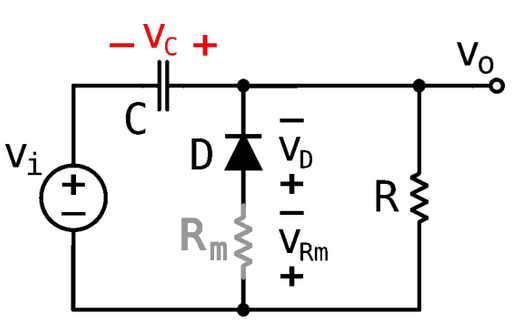
\includegraphics[width=1\columnwidth]{images/o_circuito.png}
    \caption{Circuito com diodo em configuração de grampeador.}
\end{figure}

\newpage
\subsection{Análise simbólica}

A análise é conduzida, examinando-se cada estado do diodo separadamente. O processo tem início com o diodo polarizado diretamente, seguido pelo diodo polarizado reversamente.

\subsubsection{Estado 1: Polarizacao direta}

\begin{figure}[h]
    \centering
    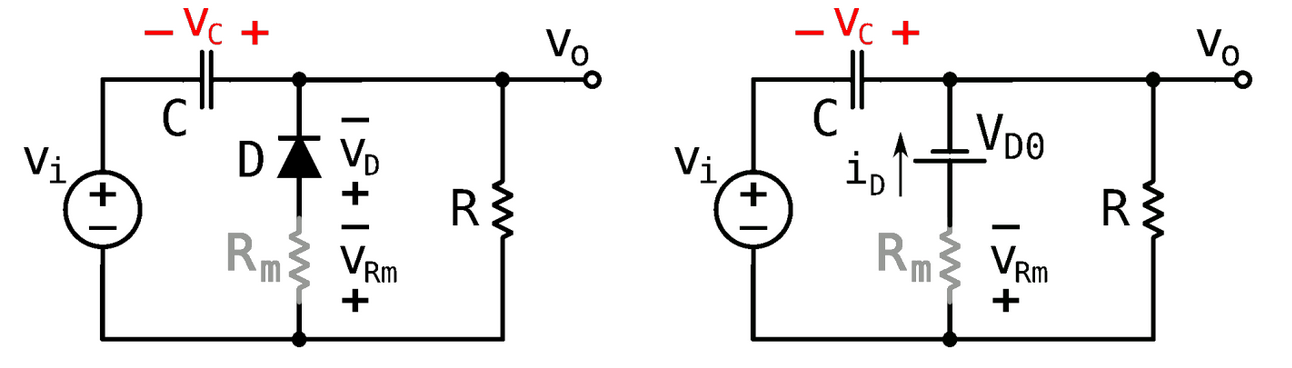
\includegraphics[width=1\columnwidth]{images/o_circuito_direto.png}
    \caption{Circuito grampeador de tensao em configuração de polarizacao direta.}
\end{figure}

Esse estado é alcançado quando o diodo está "ligado".

Nesse caso, existem restrições.

\begin{equation}
    \begin{aligned}
         & I_d > 0      \\
         & V_d = V_{D0}
    \end{aligned}
\end{equation}

A lei de Kirchhoff é aplicada ao nó denominado $V_o$.

\begin{equation}
    \frac{V_o}{R} + \frac{V_o - ( - V_{D0})}{R_m} + C \deriv{V_c}{t} = 0
\end{equation}

Observa-se que:

\begin{equation}
    V_c = V_o - V_i
\end{equation}

\begin{equation}
    \deriv{V_c}{t} + \left( \frac{1}{R_m} + \frac{1}{R} \right) \frac{V_o}{C} = - \frac{V_{D0}}{R_m C}
\end{equation}

A equação é rearranjada:

\begin{equation}
    \deriv{V_c}{t} + \left( \frac{1}{R_m} + \frac{1}{R}\right) \frac{V_o}{C} = - \frac{V_{D0}}{R_m C}
\end{equation}

Como $V_c$ é igual a $V_o - V_i$, obtém-se:

\begin{equation}
    \label{eq:diff_eq1}
    \deriv{V_o}{t} + \frac{1}{C} \left(\frac{1}{R_m} + \frac{1}{R} \right) V_o = \deriv{V_i}{t} - \frac{V_{D0}}{R_m C}
\end{equation}
\\
A condição inicial para $V_o$ em função de $V_{C0} = v(t=0)$ é dada por $V_o(0) = V_{C0} + V_i$.

Nesta prática, são feitas duas premissas:

\begin{itemize}
    \item $R_m \ll R$. \\
    \item  $V_i$ é uma onda quadrada com amplitude $\pm V_m$ e período $T_s$.
\end{itemize}

A partir da primeira premissa, obtém-se:

\begin{equation}
    \frac{1}{R_m} + \frac{1}{R} \approx \frac{1}{R_m}
\end{equation}

E da segunda premissa, durante as transições entre $\pm V_m$, tem-se:

\begin{equation}
    \deriv{V_i}{t} = 0
\end{equation}

Pode-se então simplificar a equação \ref{eq:diff_eq1} da seguinte forma:

\begin{equation}
    \label{eq:diff_eq_estado1}
    \deriv{V_o}{t} + \frac{V_o}{R_m C}= - -\frac{V_{D0}}{R_m C}
\end{equation}

Com a condição inicial: $V_o(t = 0^{+}) = V_{C0} \pm V_m$.

\hfill

A solução da equação diferencial \ref{eq:diff_eq_estado1} é dada pela soma da solução particular e da solução homogênea, como segue:

\begin{equation}
    \tag*{Parte homogenea}
    \deriv{V_{oH}}{t} + \deriv{V_{oH}}{R_m C} = 0
\end{equation}

\begin{equation}
    \tag*{Solucao generica}
    V_{oH}(t) = K e^{-\frac{t}{R_m C}}
\end{equation}

Com $K$ determinado pelas condições iniciais.

Por substituição, determina-se que uma solução particular pode ser obtida por:

\begin{equation}
    V_{oP}(t) = - V_{D0}
\end{equation}

Assim, tem-se a solução completa como:

\begin{equation}
    \tag*{Solucao completa}
    V_o(t) = K e^{-\frac{t}{R_m C}} - V_{D0}
\end{equation}

Como a condição inicial é $V_o(0) = V_{C0} \pm V_m$, a solução completa é dada por:

\begin{equation}
    \label{eq:vo_estado1}
    V_o(t) = (V_{C0} \pm V_m + V_{D0}) e^\frac{-t}{R_m C} - V_{D0}
\end{equation}

Como $V_c = V_o - V_i$, temos a seguinte solução para $V_c(t)$:

\begin{equation}
    \label{eq:vc_estado1}
    V_c(t) = (V_{C0} \pm V_m + V_{D0}) e^\frac{-t}{R_m C} \mp V_m - V_{D0}
\end{equation}

Dessa forma, obtém-se a constante de tempo $\tau_1 = R_m C$.

Das restrições desse estado, tem-se que:

\begin{equation}
    I_D = \frac{V R_m}{R_m} = - \frac{V_i + V_c + V_{D0}}{R_m} > 0
\end{equation}

Logo:

\begin{equation}
    V_i + V_c < - V_{D0}
\end{equation}

Com base nisso, as equações que regem as tensões $V_c$ (Equação \ref{eq:vc_estado1}) e $V_o$ (Equação \ref{eq:vo_estado1}) no estado 1 são obtidas.


\subsubsection{Estado 2: Polarizacao reversa}


\begin{figure}[h]
    \centering
    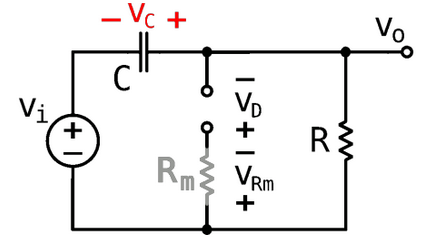
\includegraphics[width=1\columnwidth]{images/o_circuito_reverso.png}
    \caption{Circuito grampeador de tensao em configuração de polarizacao reversa.}
\end{figure}

Esse estado é alcançado quando o diodo está "desligado".

Nesse caso, existem restrições.

\begin{equation}
    \begin{aligned}
         & V_D < V_{D0} \\
         & I_D = 0
    \end{aligned}
\end{equation}

Nesse estado, observa-se que é um simples circuito RC com a tensão de saída medida sobre o resistor R.

Observa-se que $V_r = - R_{ic} = - R C \deriv{V_c}{t}$, e a equação que governa o circuito é dada por:

\begin{equation}
    V_i + V_c + R C \deriv{V_c}{t} = 0
\end{equation}

Considerando que $V_c = V_o - V_i$, podemos concluir que:

\begin{equation}
    V_o = - R C \left( \deriv{V_o}{t} - \deriv{V_i}{t} \right)
\end{equation}

Isso pode ser rearranjado em:

\begin{equation}
    \deriv{V_o}{t} + \frac{V_o}{R C} = \deriv{V_i}{t}
\end{equation}

A entrada $V_i$ é uma onda quadrada, o que implica que $\deriv{V_i}{t} = 0$, simplificando assim a equação para:

\begin{equation}
    \deriv{V_o}{t} + \frac{V_o}{R C} = 0
\end{equation}

A condição inicial é $V_o(t=0^{+}) = \pm V_m + V_{C0}$.

Portanto, a solução para $V_o$ é:

\begin{equation}
    \label{eq:vo_estado2}
    V_o(t) = (\pm V_m + V_{C0}) e^{\frac{-t}{R C}}
\end{equation}

Como $V_c = V_o - V_i$, temos a seguinte solução para $V_c(t)$:

\begin{equation}
    \label{eq:vc_estado2}
    V_c(t) = (\pm V_m + V_{C0}) e^{\frac{-t}{R C}} \mp V_m
\end{equation}

Dessa forma, obtém-se a constante de tempo $\tau_2 = R C$.

Como $R_m \ll R$, pode-se observar que $\tau_1 \ll \tau_2$.

